% TO-DO:
% * slides to mention big achievements, 附件

\documentclass[16pt]{beamer}
% \geometry{papersize={5in,4.5in}}

\ifdefined\chinchin
\usepackage[CJKspace]{xeCJK}
%\setCJKmainfont[BoldFont=SimHei,ItalicFont=AR PL KaitiM GB]{Alibaba PuHuiTi}
\setCJKmainfont{Alibaba PuHuiTi}
\newcommand{\cc}[2]{#1}
\else
\newcommand{\cc}[2]{#2}
% \renewcommand{\baselinestretch}{0.8} 
\fi

%\usepackage{newtxtext,newtxmath}	% use Times Roman font
%\usepackage{newtxtext}
%\renewcommand{\familydefault}{\sfdefault}
\usefonttheme{serif}
\usefonttheme{professionalfonts}
%\setbeamertemplate{theorems}[numbered]
\setbeamertemplate{caption}{\insertcaption} 	% no `Figure' prefix before caption

\mode<presentation> {

%\usetheme{default}
%\usetheme{AnnArbor}
%\usetheme{Antibes}
%\usetheme{Bergen}
%\usetheme{Berkeley}
%\usetheme{Berlin}
%\usetheme{Boadilla}
%\usetheme{CambridgeUS}
%\usetheme{Copenhagen}
%\usetheme{Darmstadt}
%\usetheme{Dresden}
%\usetheme{Frankfurt}
%\usetheme{Goettingen}
%\usetheme{Hannover}
%\usetheme{Ilmenau}
%\usetheme{JuanLesPins}
%\usetheme{Luebeck}
\usetheme{Madrid}
%\usetheme{Malmoe}
%\usetheme{Marburg}
%\usetheme{Montpellier}
%\usetheme{PaloAlto}
%\usetheme{Pittsburgh}
%\usetheme{Rochester}
%\usetheme{Singapore}
%\usetheme{Szeged}
%\usetheme{Warsaw}

%\usecolortheme{albatross}
%\usecolortheme{beaver}
%\usecolortheme{beetle}
%\usecolortheme{crane}
%\usecolortheme{dolphin}
%\usecolortheme{dove}
%\usecolortheme{fly}
%\usecolortheme{lily}
\usecolortheme{orchid}
%\usecolortheme{rose}
%\usecolortheme{seagull}
%\usecolortheme{seahorse}
%\usecolortheme{whale}
%\usecolortheme{wolverine}		% Hofstra

%\setbeamertemplate{footline} % To remove the footer line in all slides uncomment this line
\setbeamertemplate{footline}[page number] % To replace the footer line in all slides with a simple slide count uncomment this line
\setbeamertemplate{navigation symbols}{} % To remove the navigation symbols from the bottom of all slides uncomment this line
}

\setbeamertemplate{headline}{}
% \setbeamersize{text margin left=1mm,text margin right=1mm} 
% \settowidth{\leftmargini}{\usebeamertemplate{itemize item}}
% \addtolength{\leftmargini}{\labelsep}
% \setbeamertemplate{enumerate subitem}{(\roman{enumii})}
% \setbeamertemplate{itemize items}[default]
\setbeamertemplate{items}[square]
\setbeamertemplate{enumerate items}[default]

\usepackage[backend=biber,style=numeric]{biblatex}
\bibliography{../../AGI-book}
% \renewcommand*{\bibfont}{\footnotesize}
\setbeamertemplate{bibliography item}[text]

\usepackage{graphicx} % Allows including images
\usepackage{tikz-cd}
\usetikzlibrary{decorations.pathmorphing}
% \usepackage{tikz}
\usepackage[export]{adjustbox}% http://ctan.org/pkg/adjustbox
\usepackage{verbatim} % comments
\usepackage[skins,theorems]{tcolorbox}

\usepackage{ulem}
\makeatletter
\newcommand{\cthickuline}[3][0.5pt]{%
	\UL@protected\def\temp@uline{\bgroup\markoverwith
		{\textcolor{#2}{\rule[-0.5ex]{2pt}{#1}}}\ULon}%
	\temp@uline{#3}%
}
\makeatother

% \usepackage{tikz-cd}  % commutative diagrams
% \newcommand{\tikzmark}[1]{\tikz[overlay,remember picture] \node (#1) {};}
% \usepackage{booktabs} % Allows the use of \toprule, \midrule and \bottomrule in tables
% \usepackage{amssymb}  % \leftrightharpoons
% \usepackage{wasysym} % frownie face
% \usepackage{newtxtext,newtxmath}	% Times New Roman font
% \usepackage{sansmath}

\newcommand{\emp}[1]{\textbf{\color{violet}#1}}
\newcommand{\vect}[1]{\boldsymbol{#1}}
\newcommand{\tab}{\hspace*{1cm}}
\newcommand*\confoundFace{$\vcenter{\hbox{\includegraphics[scale=0.2]{../../confounded-face.jpg}}}$}
\newcommand{\smiley}{$\vcenter{\hbox{\includegraphics[scale=0.05]{../../smiling-face.png}}}$}

\makeatletter
\renewcommand{\boxed}[1]{\fbox{\m@th$\displaystyle\scalebox{0.9}{#1}$} \,}
\makeatother

%----------------------------------------------------------------------------------------
%	TITLE PAGE
%----------------------------------------------------------------------------------------

\title[AGI and categorical logic]{{Paper: AGI from the perspectives of categorical logic and algebraic geometry}}
\author{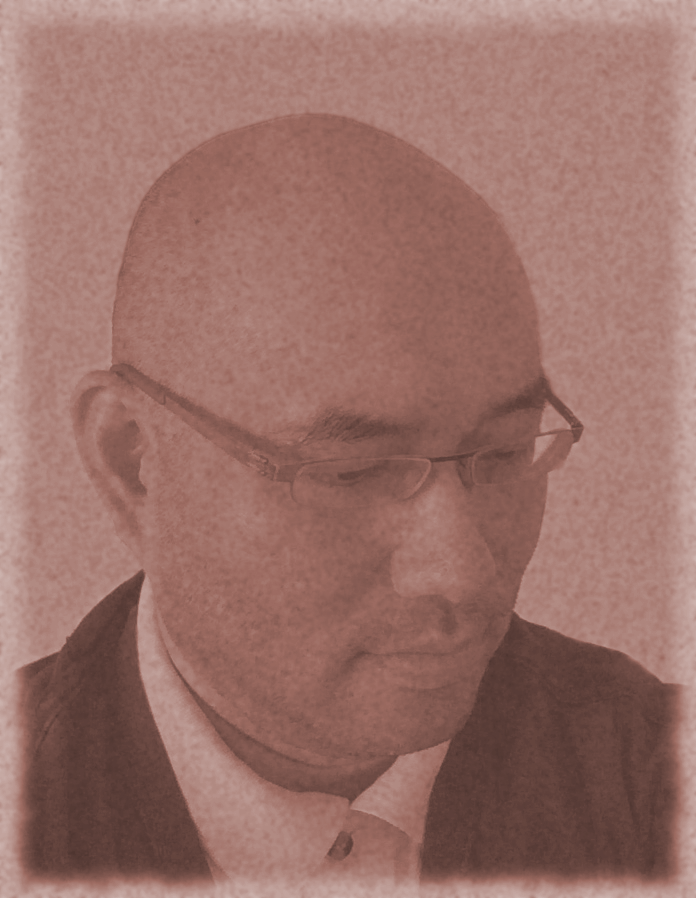
\includegraphics[scale=0.14]{John_Grothendieck.png} \\ \centering YKY}
\date{\today} % Date, can be changed to a custom date

\begin{document}

\addtocounter{page}{-1}
\begin{frame}[plain,noframenumbering]
\titlepage
\end{frame}

\addtocounter{page}{-1}
\begin{frame}[noframenumbering]
\frametitle{Contents}
\tableofcontents
% \vspace*{0.5cm}
% 多谢 支持 \smiley
\end{frame}

%----------------------------------------------------------------------------------------
%	PRESENTATION SLIDES
%----------------------------------------------------------------------------------------

\section{How does ``No Free Lunch'' guide us to accelerate AGI?}
\subsection{The hypothesis space, ie. the space of AGIs}
\subsection{A motivating example: symmetric NNs}
\subsection{Dumb structures and dumb knowledge}
\section{Categorical logic vs algebraic logic}
\section{Fibrations in particular}

\part{How does ``No Free Lunch'' guide us to accelerate AGI?}
\frame{\partpage}

\begin{frame}
\frametitle{The hypothesis space, ie. the space of AGIs}

In deep learning, our hypothesis space = neural networks = parameter space = weight space = $\mathbb{R}^n$ or $[0,1]^n$ if truncated.

It looks like this:
\begin{equation}
\vcenter{\hbox{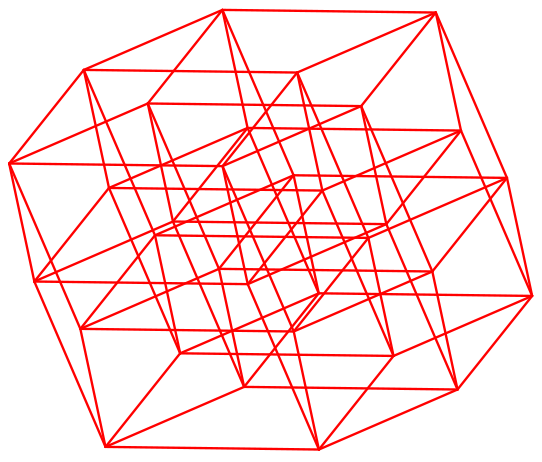
\includegraphics[scale=0.3]{hypercube.png}}}
\nonumber
\end{equation}

Imagine a loss function as sitting above this space;  We seek to minimize it by gradient descent.
\end{frame}

\begin{frame}
\frametitle{What can ``No Free Lunch'' say about the space of AGIs?}
\begin{itemize}
	\item We believe a fair coin toss has probability 1/2 by making an \textbf{ignorance assumption} and applying the maximum entropy principle.  The ignorance assumption says that we have no reason to believe that one side of the coin is more probable than the other.

	\item By a similar argument, 
		\begin{equation}
		\vcenter{\hbox{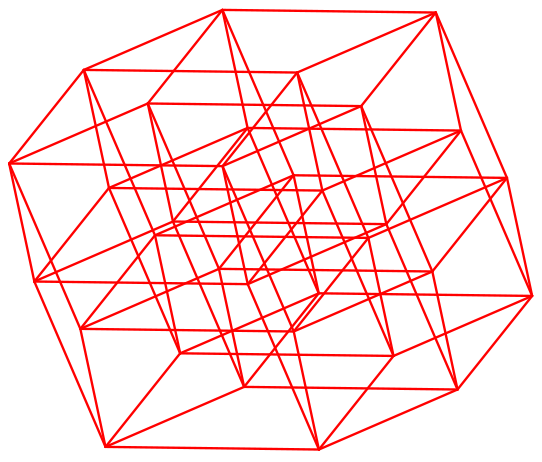
\includegraphics[scale=0.15]{hypercube.png}}}
		\nonumber
		\end{equation}
\end{itemize}
\end{frame}

\begin{frame}
	\frametitle{Unreasonable effectiveness of gradient descent}
	
	\begin{columns}
		\begin{column}{0.8\textwidth}
			\begin{itemize}
			\item Gradient descent can keep going down \textit{for a long time} as there are millions of dimensions.
			\item The ``unreasonable'' effectiveness of gradient descent in deep learning is currently our most powerful weapon to solve the AGI problem.  \\
			Its explanation is likely very difficult, as it hinges on the P =? NP problem.
			\end{itemize}
		\end{column}

		\begin{column}{0.2\textwidth}  %%<--- here
			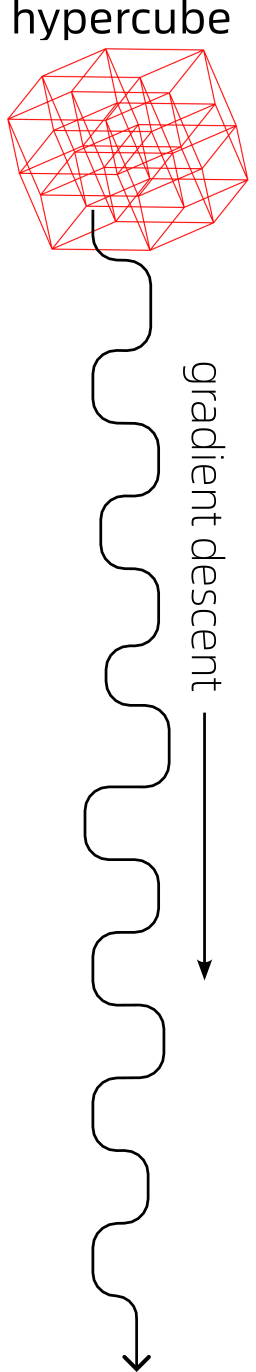
\includegraphics[scale=0.45]{gradient-descent-from-hypercube.png}
		\end{column}
	\end{columns}
\end{frame}

\begin{frame}
\frametitle{The hypothesis space has plenty of ``dumb structures''}
\begin{itemize}
	\item It seems that dumb learning-machine structures (animals) are more common than smart ones
\end{itemize}

\centering
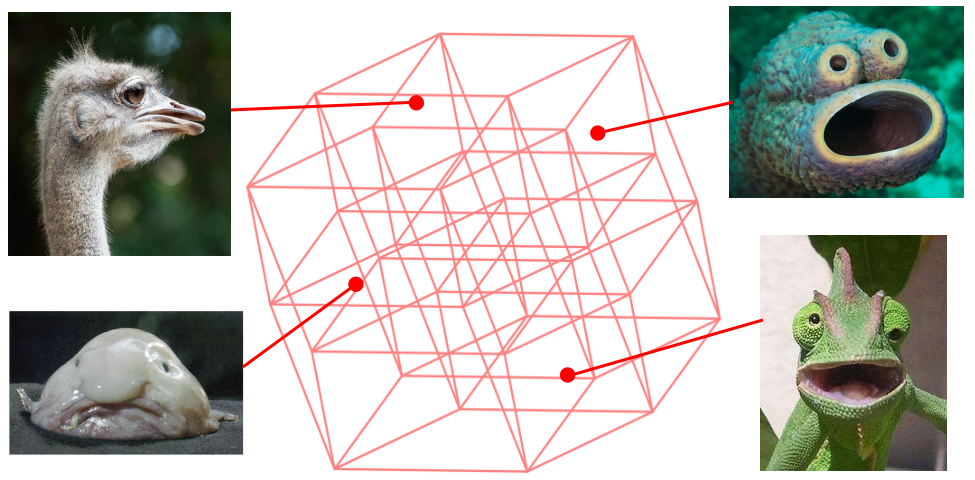
\includegraphics[scale=0.35]{dumb.png}
\end{frame}

\begin{frame}
	\frametitle{Even if we have found an intelligent structure, it may still contain lots of ``dumb knowledge'' in that sub-space}
\begin{itemize}
	\item It also seems that dumb knowledge is more common than smart knowledge
\end{itemize}

\centering
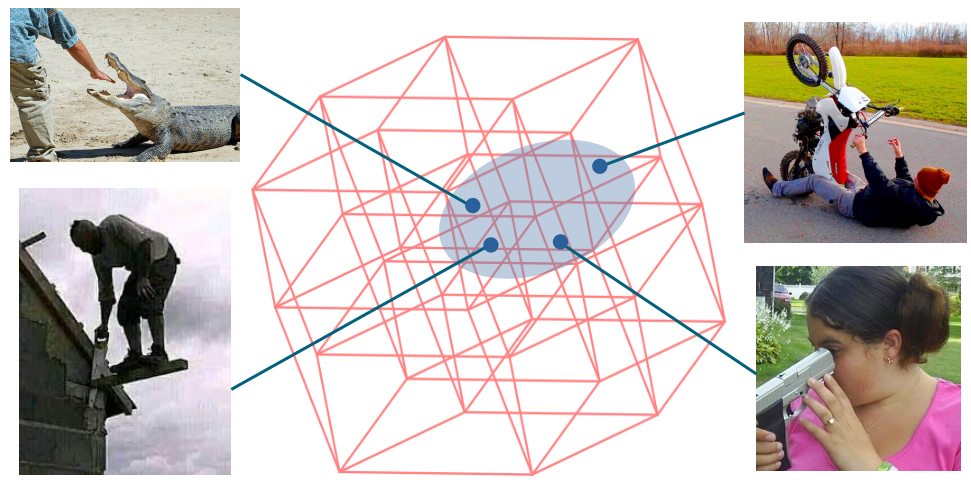
\includegraphics[scale=0.35]{dumb-behavior.png}
\end{frame}

\begin{frame}
\frametitle{A motivating example: symmetric neural networks}
\fontsize{10pt}{8}\selectfont
\begin{itemize}
	\item Permutation symmetry or commutativity ($ab = ba$) is the best-known symmetry in mathematics
	\item The input space, as a hypercube, is symmetric under exchange of vertices. The \textbf{fundamental domain} of this symmetry is one \textit{corner} of the hypercube:
	\begin{equation}
	\vcenter{\hbox{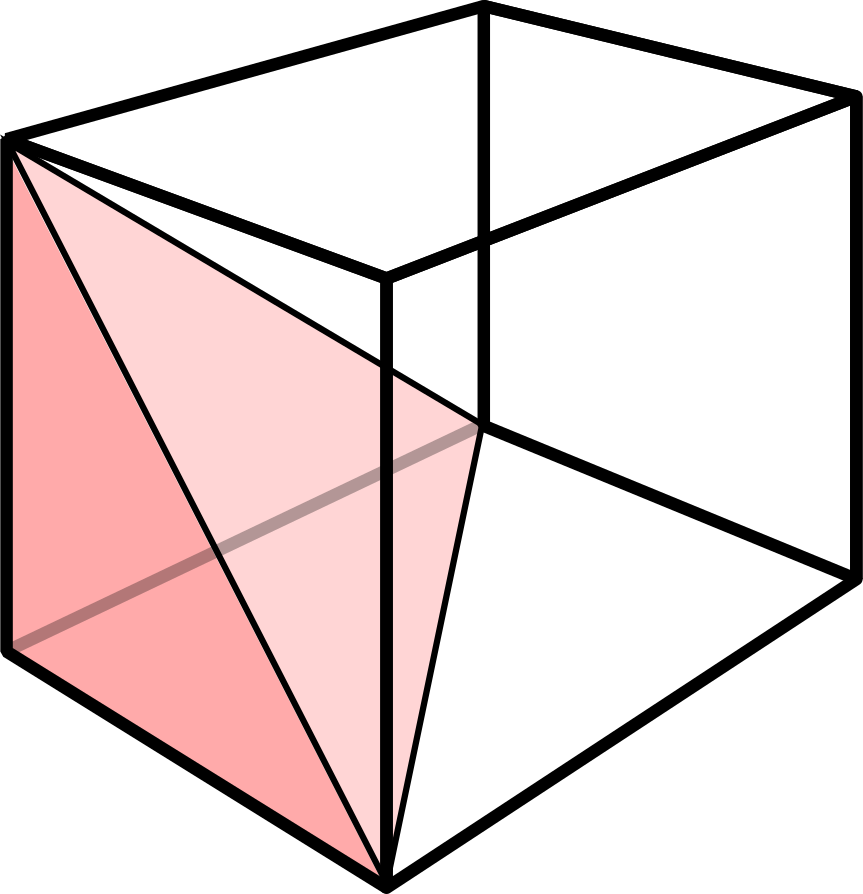
\includegraphics[scale=1]{cube-corner.png}}}
	\end{equation}
	(Note that this hypercube is the \textit{input} space, not the mapping / hypothesis space)
	\item Building a symmetry into a neural network may seem a daunting task, but recent research shows that merely \textbf{projecting} all data points to the fundamental domain has the same effect as achieving symmetry \cite{Aslan2023}.
\end{itemize}
\end{frame}

\begin{frame}
	\frametitle{A motivating example: symmetric neural networks}
	\begin{itemize}
		\item If we restrict to binary logic, the total number of Boolean functions in $n$ variables is $2^{2^n}$ whereas the number of \textbf{symmetric} Boolean functions is $2^{n+1}$.  So we clearly see an \textit{exponential} reduction in the size of the hypothesis space.
		
		\item Tantalizingly, the Transformer also has this permutation symmetry, and researchers have proposed that Transformers are capable of performing \textit{syntactic} manipulations similar to those in proofs of symbolic / predicate logic.
		
		\item We can further relax the restriction of binary logic to $k$-ary logic, ie, increase the number of lattice points in the hypercube, and the above analysis still holds qualitatively.
	\end{itemize}
\end{frame}

\part{Categorical logic vs algebraic logic}
\frame{\partpage}

\begin{frame}
\frametitle{Curry-Howard isomorphism}
Many readers may be familiar with this already, so I'll just highlight some interesting points...
\begin{itemize}
	\item The starting point of the Curry-Howard isomorphism is to make the following identification:
	\begin{equation}
		\boxed{implication in logic} A \rightarrow B \qquad A \stackrel{f}{\rightarrow} B \; \boxed{function in type theory}
		\nonumber
	\end{equation}
	\item An example in type theory: ``\textbf{currying}'' means to convert a 2-argument function into a single-argument function which returns another function, ie. $f(x,y) = (g(x))(y)$.  \\
	The types of $f$ and $g$ are equivalent, ie, $X \rightarrow (Y \rightarrow Z) \simeq (X \times Y) \rightarrow Z$. \\
	If we treat the above as logic it becomes: $X \rightarrow (Y \rightarrow Z) \equiv (X \wedge Y) \rightarrow Z$.  One can verify this is a valid logic formula.
	\item This an other amazing coincidences led us to believe that CHI has some deep truth in it.
\end{itemize}
\end{frame}

\begin{frame}
\frametitle{Categorical logic \textbf{clashes} with algebraic logic}
\fontsize{10pt}{8}\selectfont
	\begin{itemize}
	\item The late Joachim Lambek proposed a ``holy trinity'' between category theory, logic, and type theory:
		\begin{equation}
		\begin{tikzcd}[row sep=1.5em,ampersand replacement=\&]
			\& \boxed{category theory} \arrow[dr,dash] \\
			\boxed{logic} \arrow[ur,dash] \arrow[rr,dash,"Curry-Howard"] \&\& \boxed{type-theory}
		\end{tikzcd}
		\nonumber
		\end{equation}
	\item But the Curry-Howard approach is fundamentally \textit{incompatible} with the \textbf{algebraic logic} approach, for example:
		\begin{equation}
		\begin{tikzcd}[row sep=2em,ampersand replacement=\&]
		\parbox{2.2cm}{\centering $f: A \rightarrow B$ \boxed{type theory}} \arrow[dr,dash,red,squiggly,"incompatible"] \& \\
		 \parbox{1.5cm}{\centering $a \rightarrow b$ \boxed{logic}} \arrow[u,"Curry-Howard"] \arrow[r] \& \parbox{1.8cm}{\centering $a + ab = 0$ \boxed{algebraic logic}}
		\end{tikzcd}
		\nonumber
		\end{equation}
	\item I have been working in the Curry-Howard direction because it feels more ``modern'' but lately I began to think the algebraic logic approach may have more potential for computational acceleration.
	\end{itemize}
\end{frame}

\part{Fibrations in particular}
\frame{\partpage}

\begin{frame}
\frametitle{Definition of a \textbf{fiber bundle}}
A \textbf{fiber bundle} is a tuple $\xi = (E, p, B, F)$ such that:
\begin{enumerate}[(i)]
	\item $E$ = \textbf{total space}
	\item $B$ = \textbf{base space}
	\item $F$ = a topological space called the \textbf{fiber} of $\xi$
	\item $\mathrel{\substack{E\\\downarrow \\B}  {\scriptstyle p}}$ is a continuous surjective map, called the \textbf{projection}
	\item for each point $b \in B$, the inverse image $p^{-1}(b) = F_b$, called \cthickuline[1.2pt]{red}{the \textbf{fiber over} $b$, is homeomorphic to $F$}
	\item $B$ has an opening covering $\{ U_a \}_{a \in A}$ such that for each $a \in A$, there is a homeomorphism: $\psi_a: U_a \times F \rightarrow p^{-1}(U_a)$.  \\
	If $F$ is a discrete space, then the structure $F \hookrightarrow E \stackrel{p}{\rightarrow} B$ is called a \textbf{covering} of $B$.
\end{enumerate}

The condition (vi) is just a re-phrase of (v) in the form of open sets, similar to the ``gluing'' together of charts in differential manifolds.  So the essential condition is (v).

\end{frame}

\begin{frame}
\frametitle{The ``boring'' cross product}

\begin{equation}
\vcenter{\hbox{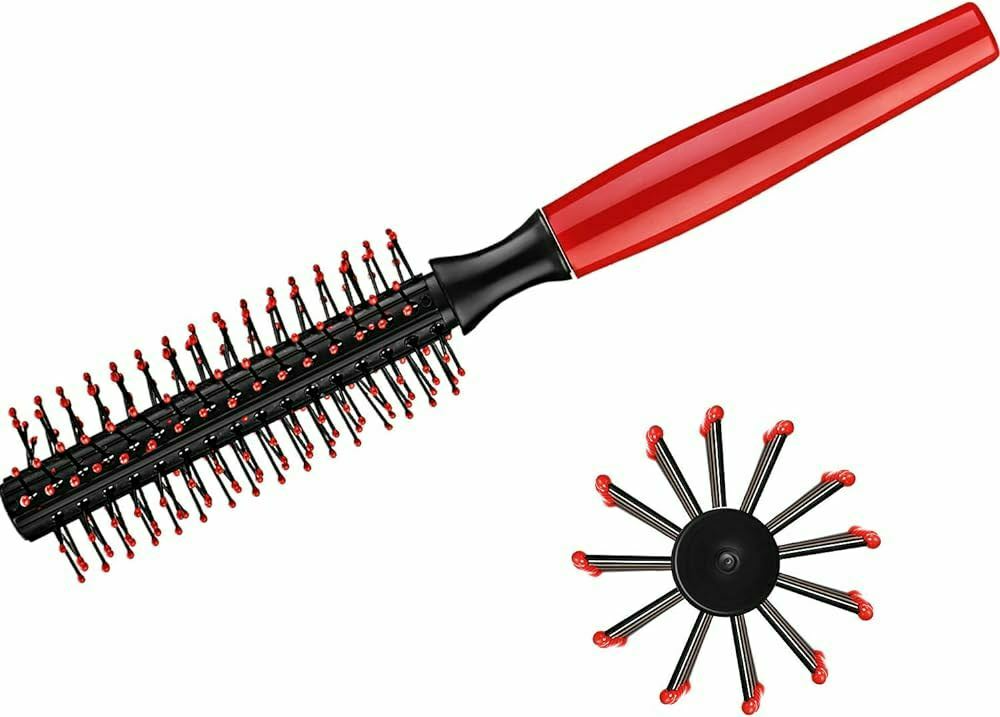
\includegraphics[scale=0.1]{hair-brush.png}}}
\nonumber
\end{equation}

\begin{equation}
	\tcbhighmath[boxrule=1pt,arc=6pt,colframe=black,shrink tight,extrude by=2mm]{token} \qquad
	\tcbhighmath[boxrule=1pt,arc=6pt,colframe=black,shrink tight,extrude by=2mm]{token} \qquad
	\tcbhighmath[boxrule=1pt,arc=6pt,colframe=black,shrink tight,extrude by=2mm]{token}
	\nonumber
\end{equation}
is equivalent to $A \times A \times A$.

\end{frame}

\part{The ``algebraic logic'' approach}
\frame{\partpage}

\begin{frame}
\frametitle{Algebraic logic}
\begin{itemize}
	\item Traditionally, algebra (and algebraic geometry) is concerned with systems of polynomials over the ``classical'' number fields $\mathbb{R}$ or $\mathbb{C}$.  The polynomials are built on addition and multiplication of numbers, that we're all familiar with.
	\item Propositional logic $(B, \wedge, \vee, \neg, \top, \bot)$ can be equated with Boolean rings $(B, \cdot, +, -, 0, 1)$, with ring multiplication identified as $\wedge$ and ring addition identified as symmetric difference (``XOR'').
	\item As predicate logic involves more operators (eg. $\forall$ and $\exists$), the classical algebra of numbers seems inadequate to represent them.
	\item For example, cylindric algebra has special operators $\mathsf{c}_i$ (cylindrification) and $\mathsf{Id}_{ij}$ (diagonal).
\end{itemize}
\end{frame}

\begin{frame}
\frametitle{Basic setup}

\end{frame}

\begin{frame}
\frametitle{References}
\cc{多谢收看}{Thanks for watching} \smiley \\
\printbibliography
\end{frame}

\end{document} 